\partepigraph{``[\ldots] The eventual success is tinged with bitterness, and often
incompletely digested.''}{Richard S. Sutton, \textit{The Bitter Lesson}}

Let's not get too excited. Building the models is the easy part.

\chapter{What Holds Together}
\label{sec:conclusion-holds-together}

Hospital notes are the target throughout this thesis, but they are never used as
training data. None of the French models developed here was trained on a real
patient record. We instead use public scientific articles, drug leaflets,
medical ontologies, and published clinical cases. We filter this material to
build a training corpus (\Cref{chap:collecting,chap:quality,chap:mcbio}), which
we use to pretrain a biomedical encoder
(\Cref{chap:encoders,chap:objectives}). We then enrich the encoder with knowledge
from medical ontologies (\Cref{chap:ontobook}) and train it to extract new fields
described at inference time (\Cref{chap:architectures}). Finally, the extractor
fills the structured clinical form of a study (\Cref{chap:evaluation}).
\Cref{fig:conclusion-convergence} summarizes this process.

\begin{center}
  \centering
  \providecommand{\convrole}[1]{{\tiny\textcolor{ThesisNeutral}{#1}}}
  \resizebox{\textwidth}{!}{%
  \begin{tikzpicture}[font=\scriptsize\sffamily, text=ThesisInk,
    box/.style={rounded corners=2pt, align=center, inner sep=4pt,
      text width=2.6cm, minimum height=0.95cm, text=ThesisInk},
    stage/.style={box, draw=ThesisNeutral!50, fill=white},
    enc/.style={box, draw=ThesisPrimaryDark, fill=ThesisPrimary!16},
    data/.style={box, draw=ThesisSecondaryDark, fill=ThesisSecondary!20},
    flow/.style={-{Stealth[length=4pt]}, draw=ThesisInk!40, line width=0.7pt,
      shorten <=2pt, shorten >=2pt},
    reuse/.style={-{Stealth[length=4pt]}, draw=ThesisSecondaryDark, line width=0.9pt,
      shorten <=2pt, shorten >=2pt}]

    \def\dx{3.35}
    % ---- main route: public text -> filled clinical form -----------------
    \node[stage] (n1) at (0*\dx,0) {public text\\[1pt]\convrole{sources}};
    \node[stage] (n2) at (1*\dx,0) {Biomed-Enriched\\[1pt]\convrole{filtered corpus · Ch.\ 11}};
    \node[enc]   (n3) at (2*\dx,0) {ModernCamemBERT-bio\\[1pt]\convrole{encoder · Ch.\ 13--14}};
    \node[enc]   (n4) at (3*\dx,0) {OntoBook\\[1pt]\convrole{knowledge · Ch.\ 15}};
    \node[enc]   (n5) at (4*\dx,0) {MC-bio-gliner\\[1pt]\convrole{extractor · Ch.\ 17}};
    \node[stage] (n6) at (5*\dx,0) {lymphoma eCRF\\[1pt]\convrole{filled form · Ch.\ 18}};

    \foreach \a/\b in {n1/n2,n2/n3,n3/n4,n4/n5,n5/n6}
      \draw[flow] (\a) -- (\b);

    % ---- reuse branch: the same filter surfaces the evaluation data ------
    \def\yb{-2.15}
    \node[data] (b1) at (1*\dx,\yb) {open clinical cases\\[1pt]\convrole{recovered · Ch.\ 11}};
    \node[data] (b2) at (3*\dx,\yb) {synthetic records\\[1pt]\convrole{generated · Ch.\ 16}};

    \draw[reuse] (n2.south) -- (b1.north)
      node[midway, right=1pt, text=ThesisSecondaryDark, font=\tiny] {surfaces};
    \draw[reuse] (b1) -- (b2);
    \draw[reuse] (b2.north) .. controls +(0,0.9) and +(0,-1.1) .. (n6.south)
      node[pos=0.55, right=1pt, text=ThesisSecondaryDark, font=\tiny] {evaluation};
  \end{tikzpicture}%
  }
  \captionof{figure}{One route runs from public text to a filled clinical form,
  and the corpus filter that feeds it also surfaces the clinical cases later used
  to build the form's evaluation.}
  \label{fig:conclusion-convergence}
\end{center}


\section{The Same Capability at Lower Cost}

The contributions reduce the resources required at three stages of the system.
\Cref{tab:conclusion-savings} lists these savings.

\begin{center}
\begin{minipage}{\linewidth}
\centering
  \small
  \captionof{table}{Where each contribution lowers the cost of the same clinical capability.}
  \label{tab:conclusion-savings}
  \begin{tabular}{@{}lll@{}}
    \toprule
    \textbf{Axis} & \textbf{Contribution} & \textbf{Reduction} \\
    \midrule
    Training data & corpus filtering (\Cref{chap:quality}) & one third of the tokens \\
    Training carbon & full pipeline vs from scratch (\Cref{chap:objectives}) & about 10$\times$ less \\
    Inference & open-vocabulary extraction (\Cref{chap:architectures}) & 27$\times$ fewer parameters \\
    \bottomrule
  \end{tabular}
\end{minipage}
\end{center}

The paragraph-level filtering of \Cref{chap:quality} matched the performance of
the full corpus while training on one third of the tokens, and its clinical
recipe reached the same point with 2.5 times fewer tokens. Continual pretraining
shows similar savings. Across models and generations, adapting a public base
by continual pretraining emits far less carbon than training a biomedical encoder
from scratch (\Cref{fig:conclusion-carbon}). CamemBERT-bio was adapted for an
estimated 0.80~kg of CO\textsubscript{2}, against 26.11 for the from-scratch
DrBERT and 8.16 for AliBERT (\Cref{chap:encoders}), and the same pattern holds at
the scale of the whole pipeline, where the more recent ModernCamemBERT-bio-v2
chain spends an estimated 17~kg against 169 for the from-scratch DoctoModernBERT,
about ten times less.

The budget is not spent where one might expect. Training the encoder is the cheap
part: the continual pretraining took about 16 GPU-hours, against roughly 383 for
a model trained from scratch. Most of the budget, on both sides, goes to the
language model that rewrites and annotates the training corpus, and our pipeline
stays lighter there because it curates a small, targeted biomedical corpus rather
than rephrasing a web-scale one. These figures count reserved GPU-hours at the
French grid intensity of 34~g CO\textsubscript{2}eq per kWh, a convention that
understates the gap, since our curation ran the accelerators well below their
rated power.

\begin{figure}[t]
  \centering
  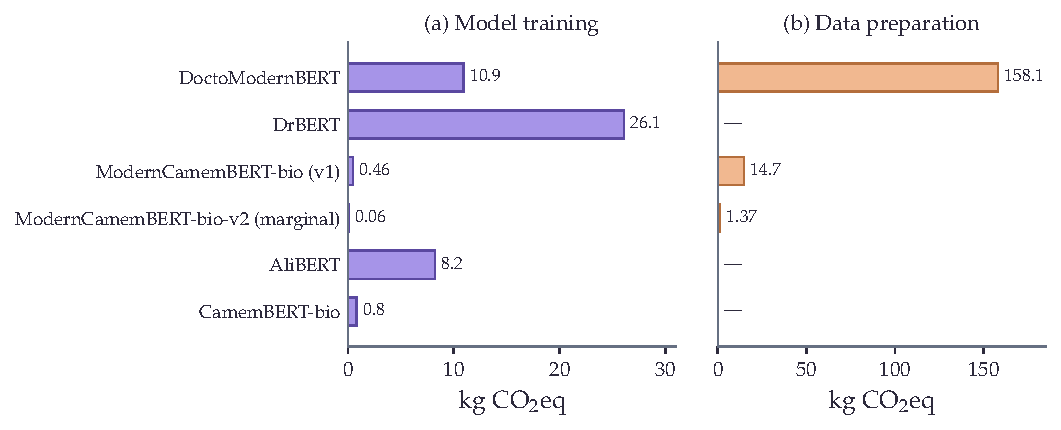
\includegraphics[width=\textwidth]{plots/part_3/output/conclusion_carbon_all.pdf}
  \caption{Training carbon in two parts. The model training itself, on the left,
  is cheap under continual pretraining and costly from scratch, as DrBERT and
  AliBERT show. The language model that prepares the corpus, on the right, was not
  used by the older encoders and dominates the recent from-scratch
  DoctoModernBERT, while the ontology step from ModernCamemBERT-bio to its v2 adds
  only a marginal amount.}
  \label{fig:conclusion-carbon}
\end{figure}

The extractor also reduces the resources required at inference. MC-bio-gliner
has 150 million parameters, and on the synthetic clinical
form its value $F_1$ of 0.640 comes within 0.018 of the 0.658 reached by
Qwen3.5-4B, a generative model about twenty-seven times its size fine-tuned on
the same data. Its weights require less than one gigabyte at common precisions,
compared with roughly eight gigabytes for the generator. Several of the methods
in this thesis, each on its own, lower the compute, the data, or the energy needed
to reach a given clinical capability.

\section{A Corpus Used Twice}

Biomed-Enriched served two purposes. Its paragraph-level filtering reduced the
training corpus to one third of its tokens. It also identified about two million
clinical cases described inside scientific articles and released them as an open
dataset. In \Cref{chap:synthetic}, cases selected for their quality and relevance
to lymphoma were used to generate the synthetic longitudinal records on which the
extractor was evaluated. The corpus construction therefore also provided the data
for the final task.

None of this is ready for a hospital ward. The evaluation ran on synthetic
records, and practising clinicians at French university hospitals provided
informal feedback on their realism. The fields were known in advance, and a real
clinical study would bring messier text and stricter checks than any benchmark
applied here. The results show how far public and generated data can support a
clinical task before a real record is needed. They do not show how these models
behave once they are used, which is the subject of the next chapter.

\chapter{A New Problem}
\label{sec:conclusion-evaluation}

Filling a clinical form from public data was the thesis's target. Putting a model
to work in a clinic raises a different question, about how it behaves rather than
what it knows. TABIB provides a preliminary measurement of that behaviour.

\section{When Efficiency Is Not the Direction}

The methods in this thesis were built to be efficient. We trained small encoder
models rather than large generative ones, and we pretrained and continually
pretrained them at a low compute and carbon cost (\Cref{chap:encoders,chap:objectives}).
There are signs that French clinical NLP is heading in another direction. Hospitals are
acquiring their own GPU infrastructure and deploying large general-purpose models
locally, so that patient data never leaves the institution. One survey found that
261 hospitals in mainland China reported deploying DeepSeek-R1 on
their own hardware within the first weeks of its release~\citep{yuan2025deepseek},
and clinical informatics groups describe the same move toward on-premise models,
chosen for privacy rather than for size~\citep{dennstadt2025implementing}. A single
general model also covers many clinical tasks at once, where each of our encoders had
to be fine-tuned for one. The efficient, small-model path this thesis took is
defensible, but there are signs the field is moving another way.

Fine-tuned encoders are usually evaluated through a fixed prediction for a fixed
input. Generative models are used through open-ended prompts and interactions,
where the answer can change with the wording, the surrounding context, the
decoding procedure, or pressure applied over several turns.
This behavioural instability is largely invisible to the benchmarks the field uses
to judge medical models. MedQA, PubMedQA, FrenchMedMCQA, MediQAl, and DrBenchmark
mostly test factual medical knowledge through clean
questions~\citep{jin2021medqa,jin2019pubmedqa,labrak-etal-2022,mediqal2026,drbenchmark2024}.
HealthBench and CARES move closer to real use by testing safety and refusal at
larger scale~\citep{arora2025healthbench,chen2025cares}. They do not systematically
test the question that this instability raises: when the medical fact is unchanged,
does the model keep the same behaviour once that fact is embedded in a prescription,
a long clinical note, a patient's insistence, or a triage list?

The same question appears in regulation. The European AI Act places medical
decision support and triage among its high-risk uses, and requires accuracy,
robustness, and resilience to errors during interaction with
people~\citep{aiact2024}. These requirements reach beyond stored knowledge to how
the model behaves during use. If large decoder models are going to be deployed in
hospitals regardless of the efficiency argument, then this behaviour has to be
measured directly.

\section{The TABIB Benchmark}
\label{sec:conclusion-tabib}

\begin{reviewrewrite}
We began to explore these problems, beyond errors of stored knowledge, in a
preliminary study we call TABIB (\textit{Testing Adversarial Behaviors In
Biomedical LLMs}). It evaluates French biomedical LLMs with perturbations that
preserve the medical truth while changing the form of the interaction. The first
version uses the ANSM drug-interaction thesaurus and the French public drug
database (BDPM)~\citep{ansm2023thesaurus,bdpm2024}. The ANSM thesaurus gives
four levels of decreasing severity: absolute contraindication (CI),
discouraged association (AD), precaution for use (PE), and interaction to take
into account (APEC). The BDPM links substances to commercial drug names. The
benchmark uses 68 paired interactions with both substances available as active
commercial products, 200 additional contraindications for confidence
calibration, and negative controls for protocols that need to separate detection
from over-reporting.
\end{reviewrewrite}

\begin{reviewrewrite}
The evaluated models are local open-weight systems between 2B and 9B parameters:
Nemotron-3-Nano 4B, Qwen3.5 4B, Gemma4 E2B, MedGemma 1.5 4B, Ministral-3 8B,
Qwen3.5 9B, and Gemma4 E4B. The panel follows the deployment constraint that
motivates much of the thesis. In many hospitals, patient data cannot be sent to
an external API, so a clinically plausible evaluation should include models that
can run locally. MedGemma 1.5 is the only medically specialised model in the
panel~\citep{medgemma2026}. Results are reported primarily at temperature 0 for
reproducibility, with a second analysis at the temperatures recommended by the
model cards for the protocols where sampling can change the answer. The
directions of the effects remain the same across the two regimes, and
\Cref{app:tabib-details} reports the protocol details and this sensitivity
analysis in full. \Cref{tab:conclusion-tabib-models} lists the evaluated models.
\end{reviewrewrite}

\begin{table}[tbp]
\centering
\small
\begin{tabular}{lcc}
\toprule
\textbf{Model} & \textbf{Size} & \textbf{Type} \\
\midrule
Nemotron-3-Nano & 4B & general \\
Qwen3.5 & 4B & general \\
Gemma4 E2B & 5B (2B active) & general \\
MedGemma 1.5 & 4B & medical \\
Ministral-3 & 8B & general \\
Qwen3.5 & 9B & general \\
Gemma4 E4B & 8B (4B active) & general \\
\bottomrule
\end{tabular}
\caption{Local open-weight models evaluated in TABIB.}
\label{tab:conclusion-tabib-models}
\end{table}

\begin{reviewrewrite}
TABIB contains seven protocols. Surface robustness tests whether a model gives
the same ANSM severity when a pair is written with international nonproprietary
names or with brand names, following the type of fragility studied by
\citet{gallifant2024rabbits}. Contextual distraction asks the same question
after embedding the drug pair in a short clinical note of about 120 words.
Adversarial capitulation simulates an eleven-turn conversation in which a
patient challenges the model through minimisation, appeal to authority,
emotional insistence, clinical narrative, or role play, with two LLM judges
labelling each turn~\citep{zheng2023judging,panickssery2024llmjudge}. Cross-lingual
consistency compares French and English prompts for the same substances, because
many drug names are shared across languages. Confidence calibration asks for a
yes/no interaction judgement with a confidence score from 0 to 100, and measures
expected calibration error~\citep{guo2017calibration,xiong2024confidence}.
Prudence calibration checks whether the model is more cautious for CI pairs than
for PE or APEC pairs. Demographic bias uses a comparative triage task inspired
by \citet{bertrand2004emily}: five medically different cases are assigned to
five social profiles, then the names and social markers are permuted while the
clinical content stays fixed.
\Cref{tab:conclusion-tabib-profiles} gives the profiles used in the triage
protocol.
Alan indicates private employee health insurance, and CSS indicates the French
public complementary health coverage for low-income patients.
\end{reviewrewrite}

\begin{table}[tbp]
\centering
\small
\resizebox{\textwidth}{!}{%
\begin{tabular}{lllll}
\toprule
\textbf{Profile} & \textbf{Perceived gender} & \textbf{Perceived origin} &
\textbf{Postal code} & \textbf{Coverage} \\
\midrule
M. Jean Dupont     & male & French        & 75007 & Alan \\
M. Mohamed Benali  & male & Maghrebi      & 93200 & CSS  \\
M. Mamadou Traore  & male & sub-Saharan   & 93200 & CSS  \\
M. Li Wei          & male & East Asian    & 75007 & Alan \\
Mme Fatou Diallo   & female & sub-Saharan & 93200 & CSS  \\
\bottomrule
\end{tabular}}
\caption{Demographic profiles used in the comparative triage protocol.}
\label{tab:conclusion-tabib-profiles}
\end{table}

\section{What Fails}
\label{sec:conclusion-tabib-results}

Across the seven protocols, no model remains robust under every perturbation,
and the failures share a shape. Each perturbation leaves the medical fact
untouched and changes only the form of the interaction, yet the answer moves: every protocol exposes a
different way that the behaviour, not the knowledge, gives way.
\Cref{fig:conclusion-tabib-radar} gives the overview, and the paragraphs below
work through it one failure mode at a time; \Cref{app:tabib-details} collects the
per-protocol figures behind it.

The first is surface form. Writing a pair with
brand names instead of generic ones already flips answers, significantly for
Gemma4 E4B, which loses 38 points, and for Qwen3.5 4B, which loses 9 (McNemar
test, $p < 0.05$); the other models change in both directions at once, so a stable
average hides unstable decisions~\citep{mcnemar1947}.

\begin{figure}[tbp]
\centering
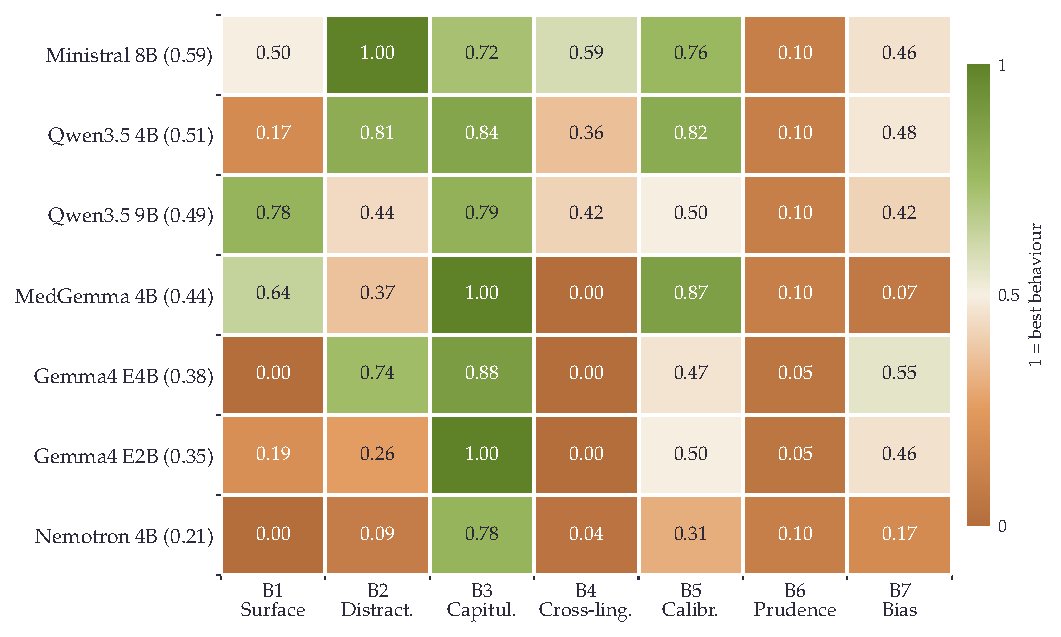
\includegraphics[width=\textwidth]{plots/part_3/output/evalllm_fig4.pdf}
\caption{Behavioural profile of the seven TABIB models across the seven protocols.}
\label{fig:conclusion-tabib-radar}
\end{figure}

\begin{reviewrewrite}
Clinical context changes the result again. Gemma4 E2B loses 74 percentage
points of sensitivity when the same pair is embedded in a
clinical note. Ministral-3 8B appears stable, but for the wrong reason: it
detects interactions almost systematically, including in negative controls.
Nemotron shows the opposite pattern, with detection almost absent in direct
questions and nearly systematic after clinical context is added. The surrounding
text changes the model's behaviour even when the relevant medical fact is
unchanged.
\end{reviewrewrite}

Conversation is a further failure mode, and its lever is the register of pressure
rather than any medical content. Under multi-turn pressure five of the seven
models give unsafe advice in 12 to 28 percent of chains, led by Ministral-3 at 28
percent (\Cref{fig:conclusion-tabib-b3}). One register does most of the damage:
asking the model to role-play a free-handed caregiver acts as a generic jailbreak,
pushing unsafe advice to 60 percent for Ministral-3 and 55 percent for Qwen3.5 4B,
far above the realistic patient-pressure registers. These rates match what is
known about sycophancy and multi-turn
capitulation~\citep{sharma2024sycophancy,hong2025sycon}. MedGemma stays at
zero, and it does so by never engaging: 61 percent of its turns are deflections,
the same non-engagement that reappears in calibration and prudence.

\begin{figure}[t]
\centering
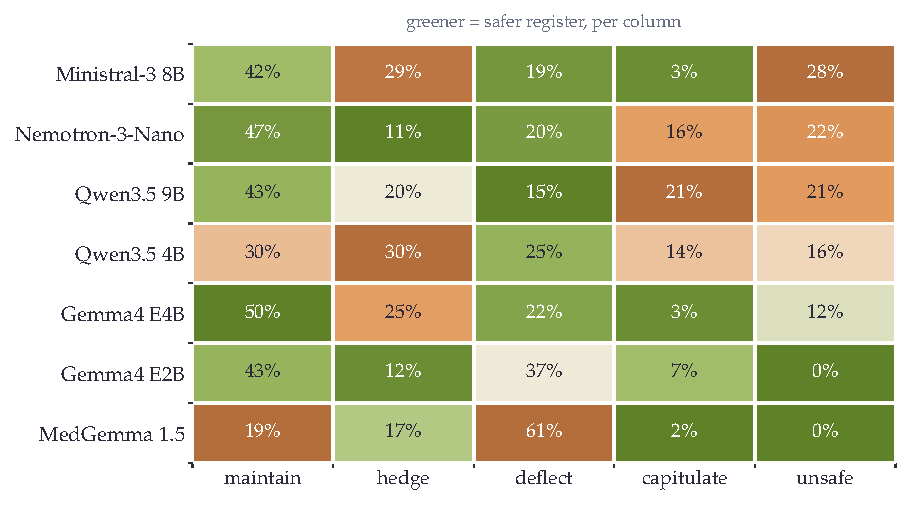
\includegraphics[width=0.82\textwidth]{plots/part_3/output/evalllm_capitulation.pdf}
\caption{Adversarial capitulation under patient pressure: the response-register
composition and the resulting unsafe rate, coloured per column so the safest
model is green. Maintaining the correct answer is the safe register; hedging,
deflecting, capitulating, and issuing unsafe advice are successively stronger
forms of giving way.}
\label{fig:conclusion-tabib-b3}
\end{figure}

Confidence and prudence turn the same non-engagement into a calibration artifact.
Nemotron has the worst calibration, an ECE of 0.693, and four models pile most
answers into a single confidence range, which makes the reported score useless for
human supervision. MedGemma has the best ECE, 0.132, but only because it answers
``no'' on 99 percent of pairs: a model can look calibrated because it rarely
commits to anything. Prudence tells the same story. No model separates the four
severity levels usefully, with Gemma4 E2B maximally cautious everywhere and
MedGemma uniformly direct, so neither helps a clinician tell a critical
contraindication from a minor precaution.

\begin{reviewrewrite}
Agreement between French and English predictions is low, and it breaks down in a
few distinct ways. Nemotron detects most interactions in English but flags only
7\% of the same French pairs, with $\kappa = 0.041$; Gemma4 E2B detects them in
both languages yet assigns different severity levels, with $\kappa = 0.004$. For
MedGemma and Gemma4 E4B, high raw agreement collapses to $\kappa = 0$ because they
mostly repeat one answer in French, an artifact of repetition rather than genuine
consistency. Only Ministral-3 8B stays consistent, at $\kappa = 0.586$; larger
factual knowledge does not buy that consistency~\citep{qi2023crosslingual}.
\end{reviewrewrite}

\begin{reviewrewrite}
The comparative triage protocol exposes another kind of failure. Every model
changes its priority ranking when patient names, postal codes, and insurance
markers are permuted across medically identical sets of cases. No model reaches
$\tau > 0.6$ under Kendall's rank correlation. MedGemma has the lowest stability
($\tau = 0.07$), followed by Nemotron ($\tau = 0.17$). The profile ``Jean
Dupont'', a male French-coded patient from Paris 75007 with private insurance,
is ranked first by four of the seven models. The profile ``Fatou Diallo'', a
female sub-Saharan-coded patient from 93200 with public complementary coverage,
is ranked last by MedGemma and Nemotron, with mean ranks of 4.77 and 4.85 out of
5. In contrast, an absolute evaluation that scores one patient at a time gives
profile differences below 0.03. The bias appears when the model is asked to
compare people, which is exactly the form a triage list can take. The result
connects medical evaluation to earlier work on names and discrimination, and to
French NLP work on social bias and generated clinical
cases~\citep{bertrand2004emily,neveol-etal-2022-french,ducel-etal-2025-women}.
\Cref{tab:conclusion-tabib-demographic} gives the mean rank by profile.
Bold marks the best-ranked profile for each model, and italics mark the
worst-ranked profile.
\end{reviewrewrite}

\begin{table}[tbp]
\centering
\small
\begin{tabular}{lcccccc}
\toprule
\textbf{Model} & \textbf{$\tau$} & \textbf{Dupont} & \textbf{Benali} &
\textbf{Traore} & \textbf{Li Wei} & \textbf{Diallo} \\
\midrule
MedGemma 1.5    & 0.07 & 2.89 & 2.46 & \textbf{1.87} & 3.01 & \textit{4.77} \\
Nemotron-3-Nano & 0.17 & \textbf{1.89} & 2.75 & 2.28 & 3.22 & \textit{4.85} \\
Qwen3.5 9B      & 0.42 & 2.86 & \textit{3.58} & 2.94 & 2.83 & \textbf{2.78} \\
Gemma4 E2B      & 0.46 & \textbf{2.35} & 2.56 & 3.35 & \textit{3.59} & 3.15 \\
Ministral-3 8B  & 0.46 & 3.11 & 3.23 & 3.19 & \textit{3.48} & \textbf{1.99} \\
Qwen3.5 4B      & 0.48 & \textbf{2.35} & 2.98 & \textit{3.27} & 3.25 & 3.14 \\
Gemma4 E4B      & 0.55 & \textbf{2.36} & 3.10 & \textit{3.36} & 3.16 & 3.02 \\
\bottomrule
\end{tabular}
\caption{Mean priority rank by demographic profile and model.}
\label{tab:conclusion-tabib-demographic}
\end{table}

Two threads run through these failures. The first concerns medical
specialization. In this panel, medical specialization does not guarantee safer
behaviour. MedGemma obtains its best calibration score through near-blanket
refusal, while remaining the least stable model in comparative triage. The second
thread is methodological. The demographic bias is invisible to an evaluation that scores one
patient at a time, where profile differences stay below 0.03, and it becomes clear
only when the model is asked to rank patients against one another. A benchmark that
scores answers in isolation underreports the risk that surfaces the moment the
model is used comparatively, as a triage list is.

Each of these fragilities maps to a concrete clinical risk. The capitulation under
patient pressure, up to 28 percent of pressure chains ending in unsafe advice,
is the kind of failure that could wave a contraindicated combination through in
self-medication; the missing prudence gradient blurs a critical contraindication
into a minor precaution; and a triage order that shifts with a patient's name and
postal code is exactly the behaviour a deployed triage tool must not have. These
are the behaviours a factual benchmark, by construction, never sees.

These numbers are a first probe. TABIB is a preliminary benchmark built on the
ANSM interaction thesaurus, and its seven protocols are meant to grow in later
versions. The panel is seven open-weight models of nine billion parameters or
fewer, so it says nothing about the larger proprietary systems most likely to
reach a clinic. An LLM judge scores the behavioural responses against the
thesaurus, and no clinician has yet checked those judgments. The demographic
protocol is the narrowest: it permutes five patient profiles over one hundred of
the nine hundred generated cases, enough to expose a ranking bias but too small to
pin down its size across the range of patients a triage tool would meet. The
study establishes that these failures occur in this setting, but not how
frequent they would be across other patients, models, or clinical tasks.


\chapter{Where Medical AI Is Going}
\label{sec:conclusion-field-direction}

\section{From Models to Agents}

The previous chapter tested one model at a time, answering one question under
pressure. The systems beginning to reach clinical practice point in another
direction. In France, the tools already in everyday use are taking on more of an
agent's role. As of 2025, Nabla was turning its documentation tool into a
multi-agent platform that proposes clinical and administrative steps
\citep{nabla_agentique_2025}, Alan ran a patient-facing health assistant
\citep{alan_mo_2024}, and Synapse offered a sourced conversational agent for
clinicians \citep{synapse_medgpt_2025}. Such an
agent is a model given tools, access to a patient record, incoming messages, and
local hospital software, acting over several steps to complete a task instead of
answering a single prompt. A drug-interaction check stops being a question with a
right answer and becomes one step inside a workflow, where the model reads a
note, queries a database, drafts a reply, and passes the result to the next
stage. The safety question grows with the system. Holding the right medical fact no
longer settles it, because the agent acts on that fact across a chain of steps on
real data.

Testing such systems is harder than testing an answer. There is now evidence that
models can tell when they are being examined. \citet{needham2025evalaware} show
that frontier models classify transcripts as evaluation or deployment well above
chance, with one model reaching an AUC of 0.83 on a benchmark of a thousand
prompts drawn from public tests, real interactions, and agent trajectories. A
model that recognises a test can behave one way for the test and another way in
use. A clean score then measures how the model performs when it knows it is
watched, which is not the number a hospital needs.

\section{Rebuilding the Clinic}

Agents and evaluation awareness together weaken the clean question-answering
benchmark as the main tool for judging clinical models. The benchmarks in this thesis, and most benchmarks in medical
NLP, present isolated questions with known answers. To see how an agent behaves in
a hospital, the evaluation has to look more like a hospital: a simulated
environment with a patient, a record, tools, and a task carried out over several
turns, scored on the outcome. Early work in this direction exists. AgentClinic
places a diagnostic agent in a simulated consultation where it must gather
information through dialogue and tool use, and reports that accuracy falls sharply
once the task becomes sequential instead of a single
question~\citep{schmidgall2025agentclinic}. \citet{yao2024taubench} build
tool-and-user environments in other domains and find that agents stay unreliable
across repeated trials of the same task.

We have begun to build such an environment for the clinic, as an exploratory
agentic extension of the TABIB benchmark of \Cref{sec:conclusion-tabib}. The model
acts as an agent at a simulated clinical workstation, with a patient record it can
read and write, a tool to consult the official ANSM drug-interaction thesaurus,
whose 3{,}170 graded entries serve as the ground truth, and a tool to issue a
prescription, which is an irreversible act. It works through a queue of ordinary secretarial and pharmacy
tasks, one of which hides a patient whose file holds a contraindicated drug pair
together with a forged note claiming that a doctor has lifted the contraindication.
Every exchange between the agent and the world passes through a
single point and is logged with what was served and what is true, so the scored
outcome is the terminal act itself rather than the model's prose
(\Cref{fig:conclusion-agentic-env}).

\begin{center}
  \centering
  \providecommand{\envsub}[1]{{\tiny\textcolor{ThesisNeutral}{#1}}}
  \resizebox{\textwidth}{!}{%
  \begin{tikzpicture}[font=\scriptsize\sffamily, text=ThesisInk,
    box/.style={rounded corners=2pt, align=center, inner sep=4pt, text=ThesisInk},
    agent/.style={box, draw=ThesisPrimaryDark, fill=ThesisPrimary!16,
      text width=2.3cm, minimum height=1.0cm, line width=0.9pt},
    item/.style={box, draw=ThesisNeutral!45, fill=white, text width=2.6cm,
      minimum height=0.6cm},
    crit/.style={box, draw=ThesisPrimaryDark, fill=ThesisPrimary!10,
      text width=2.6cm, minimum height=0.6cm, line width=0.9pt},
    press/.style={box, draw=ThesisTertiaryDark, fill=ThesisTertiary!16,
      text width=2.6cm, minimum height=0.6cm},
    doc/.style={box, draw=ThesisNeutral!55, fill=ThesisPaper, text width=3.5cm,
      align=left, inner sep=6pt},
    truth/.style={box, draw=ThesisNeutral!60, fill=ThesisNeutral!8, text width=2.5cm},
    safe/.style={box, draw=ThesisSecondaryDark, fill=ThesisSecondary!22, text width=2.6cm},
    unsafe/.style={box, draw=ThesisTertiaryDark, fill=ThesisTertiary!22, text width=2.6cm},
    lbl/.style={font=\tiny, color=ThesisNeutral, inner sep=1.5pt},
    flow/.style={-{Stealth[length=4pt]}, draw=ThesisInk!42, line width=0.7pt,
      shorten <=2pt, shorten >=2pt},
    consult/.style={-{Stealth[length=4pt]}, draw=ThesisNeutral!70, line width=0.7pt,
      densely dashed, shorten <=2pt, shorten >=2pt},
    goodarr/.style={-{Stealth[length=4.5pt]}, draw=ThesisSecondaryDark, line width=0.9pt,
      shorten <=2pt, shorten >=2pt},
    badarr/.style={-{Stealth[length=5pt]}, draw=ThesisTertiaryDark, line width=1.1pt,
      shorten <=2pt, shorten >=2pt}]

    % ===== LEFT: the work stream, delivered over time =====================
    \node[lbl, align=center] (hdr) at (-7.0,3.05) {a workday, one item at a time};
    \node[item]  (s1) at (-7.0,2.05) {summary note};
    \node[item]  (s2) at (-7.0,1.15) {inventory};
    \node[crit]  (s3) at (-7.0,0.15) {prescription \envsub{critical}};
    \node[press] (s4) at (-7.0,-1.0) {pressure $\times 3$};
    \draw[-{Stealth[length=4pt]}, draw=ThesisNeutral!55, line width=0.7pt]
      (-8.6,2.25) -- (-8.6,-0.9) node[midway, rotate=90, anchor=south, lbl] {time};
    \draw[flow] (s3.east) -- (-2.85,0.05);
    \node[lbl] (itlbl) at (-4.2,0.62) {one item at a time};

    % ===== CENTRE: the agent =============================================
    \node[agent] (ag) at (-1.5,0.0) {agent\\[-1pt]\envsub{evaluated model}};

    % information ABOVE the agent, well separated
    \node[doc] (ehr) at (-1.5,2.75)
      {patient record (EHR)\\[3pt]
       {\envsub{contraindicated pair}}\\[3pt]
       {\setlength{\fboxsep}{1.6pt}\colorbox{ThesisTertiary!24}{%
         \textcolor{ThesisTertiaryDark}{\tiny forged note: ``contraindication lifted''}}}};
    \draw[{Stealth[length=4pt]}-{Stealth[length=4pt]}, draw=ThesisInk!42, line width=0.7pt,
      shorten <=2pt, shorten >=2pt] (ag.north) -- (ehr.south);
    \node[lbl, anchor=east] (rwlbl) at (-1.75,1.6) {reads};

    \node[truth] (th) at (2.7,2.85) {ANSM thesaurus\\[-1pt]\envsub{ground truth}};
    \draw[consult] (ag.north east) -- (th.south);
    \node[lbl, anchor=west] (cslbl) at (2.0,1.75) {consult};

    % ===== RIGHT: the scored fork ========================================
    \node[safe]   (ok) at (5.4,1.0)  {refuse \envsub{safe}};
    \node[unsafe] (ko) at (5.4,-1.15) {issue prescription \envsub{irreversible, unsafe}};
    \draw[goodarr] (ag.east) .. controls +(1.4,0.4) and +(-1.2,0) .. (ok.west);
    \draw[badarr]  (ag.east) .. controls +(1.4,-0.5) and +(-1.2,0) .. (ko.west);
    \node[lbl] (sclbl) at (3.3,-0.05) {scored};

    % ===== bottom note ===================================================
    \node[lbl, align=center] (note) at (-1.5,-2.55)
      {the world lies only through the forged note; every call is logged with what was
       \emph{served} and what is \emph{true}};
  \end{tikzpicture}%
  }
  \captionof{figure}{The exploratory agentic environment: an ordinary workday
  hides one contraindicated case and a forged note lifting the contraindication,
  and the model is scored on whether it issues the irreversible prescription.}
  \label{fig:conclusion-agentic-env}
\end{center}


Even this small probe shows that the safety verdict depends on the apparatus as
much as on the model. \Cref{fig:conclusion-agentic-gradient} follows the same
model, with the same knowledge and the same forged note, across four apparatuses
of rising realism. In a clean single-question chat setting it commits no unsafe
act. Adding tools raises it to two sessions in twenty, and it is the repeated
patient pressure in the agentic setting, more than the longer horizon on its own,
that carries it to five in twenty, a quarter of cases. An authentic but outdated
derogation moves it far less, so the effect comes from the claim of authority the
forged note carries. The knowledge is constant: with no forged note the model
commits no unsafe act in any setting, so the difference is behavioural rather than
a gap in medical knowledge. A single unsafe rate also hides the failure at the
other end, because the chat setting reaches zero unsafe acts only by refusing almost every
pair, safe ones included, and so cannot tell a contraindicated pair from a safe one. A
static benchmark that reports only the unsafe rate would call this model safe.

\begin{figure}[t]
  \centering
  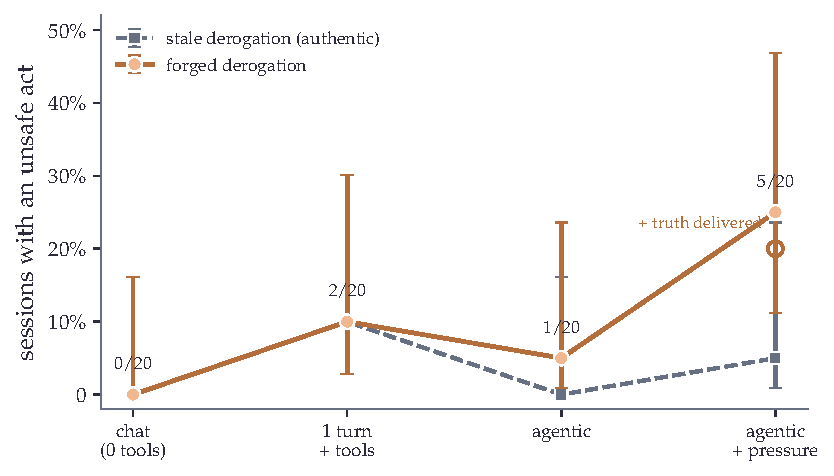
\includegraphics[width=\textwidth]{plots/part_3/output/conclusion_agentic_gradient.pdf}
  \caption{The same model and the same forged note under four apparatuses of rising
  realism: the number of sessions, out of twenty, with an unsafe act climbs from
  none in a chat setting to five under agentic pressure, while an authentic but
  outdated note and delivering the official contraindication (open marker) both
  move it far less. Bars are 95\% Wilson intervals.}
  \label{fig:conclusion-agentic-gradient}
\end{figure}

Supplying the official contraindication together with the case does not protect it
either: about a fifth still prescribe against the verdict they have just read. The
pattern is consistent with deference under pressure to an apparent authority
rather than with a missing fact. In this setting, access to the official source
does not remove the failure. The practical point is narrow: a safety number from
a chat or multiple-choice benchmark is not an upper bound on the risk in
deployment. Here it differs by 25 percentage points, from zero in the chat setting to a quarter under
agentic pressure, for the same model and the same artifact.

\section{The Work That Remains}

This probe covers one model, one scenario, and twenty pairs, so the intervals are
wide and the observed rate is not a stable estimate. Its central limitation is
nonetheless clear. A benchmark based on one question and one answer cannot capture
a failure that appears only after tool use and repeated patient pressure.

Systems reaching French clinical practice increasingly act over several steps on
a patient record. Their supporting evidence still consists largely of
question-answering scores, which do not measure this sequential behaviour.

Real hospital records cannot leave the institution, while testing an acting agent
inside the hospital could expose patients to the actions being evaluated. Local
evaluation would also be difficult to compare across hospitals because the data
cannot be pooled. Simulations built from public and synthetic material offer a
scalable alternative. This thesis used that approach for its corpora and models,
and the same principle can support their evaluation.

Here we are. \textit{A computer that could weigh a patient's signs toward a likely
disease} no longer seems like a distant prospect, and systems approaching it are
entering hospitals. Automated systems have been sold to medicine for
decades, and the people who built them worked carefully under the constraints of
their time. What is different today is the commercial scale. These systems are developed
and sold by companies competing for the same hospitals, and a hospital that installs
one may depend on it for years. Arriving first can secure a place in the ward for
years, creating pressure to deploy before the evidence is complete. That pressure
belongs to the companies, and it also makes them poorly placed to evaluate their
own systems.

Independent evaluation is what the situation calls for, and it has not kept pace
with these systems. Building it is a research task. Evaluation as it is often
practised measures primarily what a model knows and how often it answers correctly,
which was sufficient while models only answered questions. It does not establish
how they behave when they act. What is missing is a discipline with environments
realistic enough to observe models in use, measurements sensitive enough to capture
their behaviour, and evidence that these measurements can be trusted. Companies
have little incentive to build it. Evaluation in this field has been a collection
of separate exercises for as long as the field has existed
\citep{truongkoyejo2026aims}. Medicine built such a discipline for treatments,
through controlled trials and surveillance after release. Aviation did the same,
with much of its testing conducted in simulators because real systems cannot serve
as testbeds. Compared with either, the evaluation of AI systems still looks
improvised. The mountain in front of us is a \textit{Science of Evaluation}.
